\documentclass[a4paper, 12pt]{article}
% math symbols
\usepackage{amssymb}
\usepackage{amsmath}
\usepackage{mathrsfs}
\usepackage{physsummer}


\usepackage{enumitem}
\usepackage[margin = 2cm]{geometry}

\tolerance = 1000
\emergencystretch = 0.74cm



\pagestyle{empty}
\parindent = 0mm

\usetikzlibrary{hobby}

\begin{document}

\begin{center}
  \Large{\textbf{Городской центр физического образования, 10 класс.}\\
  \textit{Серия 3, 2 октября 2014.}}
\end{center}

\begin{center}
  \Large \textbf{Для разогрева.}
\end{center}

\large

\task{ В стенке сосуда с газом сделали маленькое отверстие. Как будет
  изменяться температура газа в сосуде по мере вытекания газа через
  отверстие? }

\begin{center}
  \Large \textbf{ Смеси газов.}
\end{center}

\taskpic{ В левой секции сосуда находится смесь водорода и гелия,
  причем парциальные давления водорода и гелия одинаковые. В правой
  секции сосуда --- вакуум. В перегородке на короткое время открывают
  отверстие. Каким будет отношение давлений гелия и водорода в правой
  секции?  }
{
  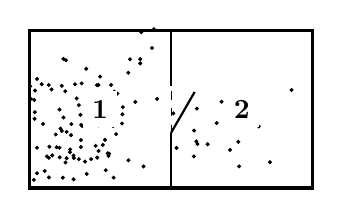
\begin{tikzpicture}
    \draw[very thick] (0.2,0) rectangle (3.8,2);
    \draw[thick] (2,0) -- (2,0.7) (2,1.3) -- (2,2);
    \draw[dashed] (2,0.7) -- (2,1.3);
    \draw[thick] (2,0.7) -- ++(60:0.6cm);% node[above] {\textbf{A}};
    \draw plot [only marks, mark=*, mark size=0.5, domain=1:2,
    samples=100] (0.2+rnd*\x,0.1+rnd*\x); 
    \draw plot [only marks, mark=*, mark size=0.5, domain=1:1.5,
    samples=15] (2.2+rnd*\x,0.1+rnd*\x);
    \draw (1.1,1) node[fill=white] {\textbf{1}};
    \draw (2.9,1) node[fill=white] {\textbf{2}};
  \end{tikzpicture}
}

\task{ В закрытом сосуде при давлении $P$ находится смесь из одного
  моля водорода и одного моля кислорода. Газ в сосуде поджигают и
  происходит реакция с образованием водяного пара. Каким будет
  давление газа в сосуде после остывания газа до первоначальной
  температуры?  }

\task{ Цилиндрический сосуд разделен подвижным, хорошо проводящим
  поршнем на две части. В начальный момент справа от поршня находится
  кислород, а слева --- смесь гелия и водорода. Масса кислорода 32
  г. Поршень при этом располагается посредине сосуда. Материал поршня,
  непроницаемый для водорода и кислорода, оказался проницаемым для
  гелия, в результате чего поршень начал перемещаться и окончательно
  расположился на расстоянии четверти длины цилиндра от левой
  стенки. Определите массы гелия и водорода в смеси. Температура
  поддерживается постоянной. }

\begin{center}
  \begin{tikzpicture}
    \draw[pattern=north east lines] (2.8,0) rectangle (3.2,3);
    \draw[very thick] (0,0) rectangle (6,3);
    \draw (1.5,1.5) node{$H_2$ + $He$};
    \draw (4.5,1.5) node{$O_2$};
  \end{tikzpicture}
\end{center}

\end{document}


%%% Local Variables: 
%%% mode: latex
%%% TeX-engine:xetex
%%% TeX-PDF-mode: t
%%% End:
